% The methods that you use goes here
We combine left-to-right HMMs defined by neural networks with normalising flows to learn the distribution over the spoken utterances conditioned on text.
\vspace{0.3cm}
\begin{center}
  \vspace{-0.4cm}
  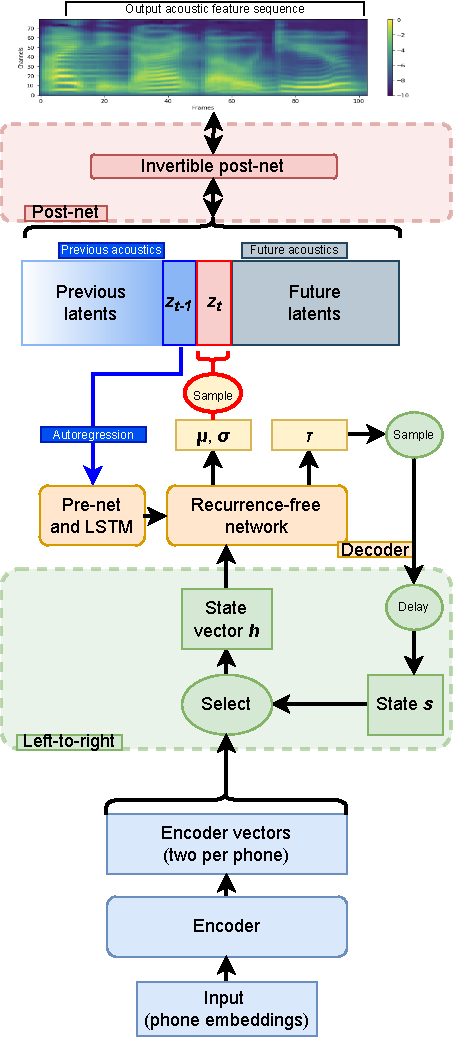
\includegraphics[height=\linewidth]{OverFlow.pdf}  
  \vspace{-0.4cm}
\end{center}
\vspace{0.25em}

Neural HMMs describe a distribution over discrete-time sequences, typically %(but not necessarily) 
assuming a Gaussian distribution for each frame.
Normalising flows,
provide a method for turning simple \emph{latent} or \emph{source} distributions $Z$, such as Gaussians, into much more flexible \emph{target} distributions $X$ through deep learning.  
The idea is to apply an invertible nonlinear transformation $f$ to the source distribution to obtain the target distribution, as $X=f(Z;\,W)$, where $f$ is parameterised by a neural network with weights $W$ and 
%To ensure invertibility we require that 
$x$ and $z$ have the same dimensionality.
%The main advantage of 
Invertibility allows us to compute the (log-)probability of %any observed outcome 
$x$ using the change of variables formula
\begin{align*}
\ln p_{X}(x)
& = \ln p_{Z}(f^{-1}(x;\,W))
+ \ln \vert \det J_{f^{-1}}(x;\,W) \vert
\text{,}
\end{align*}
where $J_{f^{-1}}(x;\,W)$ is the Jacobian matrix of $f^{-1}$ evaluated at $x$.
% \vspace{1em} % Fill in to put references at the bottom
